\documentclass[11pt]{report}
\usepackage{amssymb,amsmath}
\usepackage[utf8]{inputenc}

\usepackage[T1]{fontenc}

\usepackage[francais]{babel}
\usepackage{graphicx}
\usepackage[top=2cm, bottom=2cm, left=2cm, right=2cm]{geometry} %pour modifier les marges
\usepackage{setspace} % pour modifier les interlignes
\usepackage{array}


\renewcommand{\thesection}{\Roman{section}}
\newcommand{\deriv}{\mathrm{d}}


%création de la page de garde
\title{{\huge Signal et Filtrage - Corrections des exercices}} 
\author{Alexandre Boyer, Pascal Acco, Léa Cot, Etienne Sicard}
\date{Septembre 2019}

\begin{document}
	\maketitle
	
	\textbf{Signal \& Filtrage}
	
	\textbf{}\\
	
	2 IMACS
	
	2019 - 2020
	
	alexandre.boyer@insa-toulouse.fr	
	page Moodle
	
	
\chapter{L'étude de la réponse des systèmes linéaires à temps invariant}

	\subsubsection{Exercice 1} 
	Soient les systèmes dont le comportement temporel est défini par les équations suivantes. Indiquez si ces systèmes sont linéaires, à temps invariant et causaux ?
	
	a. $y(t) = x(t)+4\frac{dy}{dt}$ 
	
	b. $y(t) = 2x(t)+2$ 
	
	c. $y(t)=e^{-t}x(t-2)^{2}$
	
	d. $y(t)=\frac{dx}{dt}+x(t+2)$
	
	\vspace{1\baselineskip}
	

	
	\textbf{\underline{Correction exercice 1}}\\
	a. On vérifie facilement que le système est :
	 \begin{itemize}
	 	\item linéaire (soit $x_{1}(t) $ et $x_{2}(t)$ les solutions de l'équation pour $y_{1}(t)$ et $y_{2}(t)$. $x(t)=ax_{1}(t)+bx_{2}(t)$ ne peut être la solution que de $y(t)=ay_{1}(t)+by_{2}(t)$).
	 	\item à temps invariant (les paramètres de l'équation sont invariants dans le temps)
	 	\item causal (la sortie ne dépend pas des états futurs de l'entrée et de la sortie).
	 \end{itemize}
 	\vspace{0.5\baselineskip}
 	b. Le système est causal et à temps invariant, mais n'est pas linéaire. Soit  $x_{1}(t) $ et $x_{2}(t)$ les solutions de l'équation pour $y_{1}(t)$ et $y_{2}(t)$. $x(t)= ax_{1}(t)+bx_{2}(t)$ est la solution de $y(t)=2ax_{1}(t)+2+2bx_{2}(t)+2 \neq ay_{1}(t)+by_{2}(t)=2ax_{1}(t)+2a+2bx_{2}(t)+2b$
 	
 	\vspace{0.5\baselineskip}
 	c. Le système n'est ni linéaire ( $x(t)= ax_{1}(t)+bx_{2}(t)$ est la solution de $e^{-t}(ax_{1}(t-2)+bx_{2}(t-2))^{2} \neq ae^{-t}x_{1}(t-2)^{2}+be^{-t}x_{2}(t-2)^{2}$), ni à temps invariant (le coefficient devant $x^{2}$ dépend du temps). Le système est causal (la sortie à l'instant t dépend de l'entrée donnée à un instant passé (t-2)).
 	
 	\vspace{0.5\baselineskip}
 	d. Le système est linéaire et à temps invariant, mais n'est pas causal puisque la sortie à un instant t dépend de l'entrée à un instant futur (t+2).
 	
 	\vspace{1\baselineskip}
 	
 	
 	\subsubsection{Exercice 2} 
 	1. On trace les réponses de deux systèmes LTI. Proposez une expression mathématique décrivant ces réponses.
 	\begin{figure}[h!]
 		\centering
 		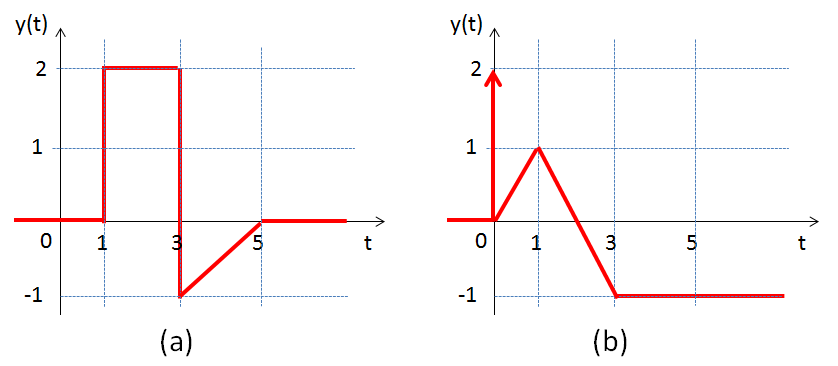
\includegraphics[scale=0.5]{images/Exo_2_2.jpg} 
 	\end{figure} \\
 
 	\vspace{0.5\baselineskip}
 	
 	2. Réécrivez sous la forme d'une fonction à valeurs réelles les fonctions suivantes et esquissez leur forme temporelle (pour t >0) :
 	
 	a. $x(t) = (1+j)e^{j\cdot 10t}$ 
 	
 	b. $y(t) = e^{(-2+j)t}\cdot u(t-2)$ 
 	
 	c. $z(t) = e^{(-1+2j)t}+e^{(-1-2j)t}$
 	
 	\vspace{1\baselineskip}	
 	
 	\subsubsection{Exercice 3 - Réponse indicielle d'un circuit RC}
 	
 	On reprend le circuit RC dont on a étudié la réponse dans la partie VI.3. On considère deux cas : celui où le condensateur est déchargé initialement, puis celui où il est chargé. 
 	
 	a. Calculez la réponse naturelle du circuit lorsque le condensateur est initialement chargé.
 	
 	b. En déduire la réponse impulsionnelle du circuit.
 	
 	c. Calculez la réponse lorsque le circuit est soumis à un échelon de Heaviside d'amplitude E, dans les deux cas (charge initiale absente ou présente).
 	
 	d. En déduire la réponse indicielle du circuit.
 	 
 	\vspace{1\baselineskip}
 	
 	\subsubsection{Exercice 4}
 	
 	On considère les deux circuits électriques ci-dessous. Pour le circuit (a), la tension initiale (t=0) aux bornes du condensateur C est notée $U_{C0}$. Pour le circuit (b), un courant noté $I_L0$ traverse la bobine L. La sortie de ces deux circuits est la tension $U_{S}$.
 	
 	\begin{figure}[h!]
 		\centering
 		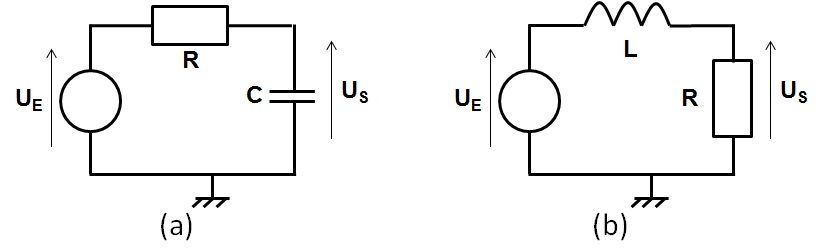
\includegraphics[scale=0.5]{images/Exo_2_4.jpg} 
 	\end{figure} 
 	
 	a. Déterminez les fréquences et les réponses naturelles de ces deux circuits. Quel est l'ordre de ces deux systèmes ? 
 	
 	b. On excite ces deux systèmes à l'aide d'un échelon de Heaviside d'amplitude notée E. Déterminez la réponse indicielle de ces deux circuits. 
 	
 	c. Déterminez les fonctions de transfert de ces deux circuits.
 	
 	\vspace{1\baselineskip}
 	
 	\subsubsection{Exercice 5 - Fonction de transfert d'un circuit résonant}
 	
 	On reprendre le circuit RLC présenté dans la partie IV.4. Celui-ci est excité par un générateur de courant I, comme le montre la figure ci-dessous. On s'intéresse à la tension U aux bornes de ce circuit RLC. 
 	 	
 	\begin{figure}[h!]
 		\centering
 		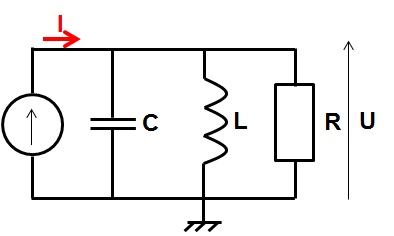
\includegraphics[scale=0.5]{images/Exo_2_5.jpg} 
 	\end{figure} 
 
 	a. Déterminez la fonction de transfert de ce circuit. 
 	
 	b. Précisez l'unité de la fonction de transfert. 
 	
 	c. Dans le cas où l'on considère une excitation cosinusoïdale du circuit, y a t-il une fréquence particulière où la réponse présente un maximum ? Si oui, laquelle ? Donnez l'expression de la réponse temporelle du circuit en régime permanent.
 	
 	\vspace{1\baselineskip}
 	
 	\subsubsection{Exercice 6}
 	
 	On considère le système dont le fonctionnement est décrit par le schéma-bloc ci-dessous. Celui-ci transforme un signal d'entrée e(t) et délivre en sortie un signal s(t). 
 	
 	\begin{figure}[h!]
 		\centering
 		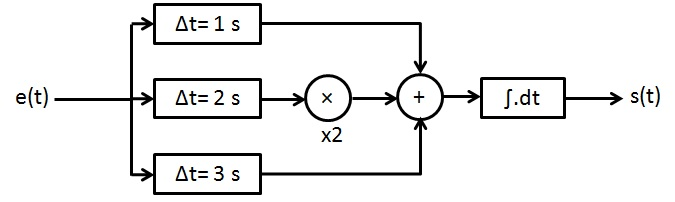
\includegraphics[scale=0.5]{images/Exo_2_6.jpg} 
 	\end{figure}
 
 	a. Le système est-il linéaire, à temps invariant, causal ?
 	
 	b. Déterminez l'expression de la réponse impulsionnelle h(t) du système. Esquissez l'allure temporelle de la réponse impulsionnelle. 
 	
 	c. Déterminez l'expression de la fonction de transfert H(p) du système. Précisez les pôles et les zéros de la fonction de transfert. Que concluez-vous sur sa stabilité ?
 
 	\vspace{1\baselineskip}
 	
 		\textbf{\underline{Correction exercice 6}}\\
 	a. Le système transforme le signal d'entrée à partir de trois opérations de base : retard, multiplication par une constante et intégration temporelle. Il s'agit d'opérations purement linéaires. Le fonctionnement du système est indépendant du temps. Il s'agit donc d'un système LTI. De plus, il est causal puisque la sortie ne dépend que des états passés du signal d'entrée.
 	
 	b. On considère une entrée égale à une impulsion de Dirac : $e(t) = \delta(t)$.	Avant l'intégrateur, le signal résultant s'écrit : $e(t-1)+2e(t-2)+e(t-3)=\delta(t-1)+2\delta(t-2)+\delta(t-3)$. L'impulsion de Dirac résultant de la dérivée de l'échelon de Heaviside, après intégration, la sortie du système est donnée par : $s(t) = h(t) = u(t-1)+2u(t-2)+u(t-3)$.
 	
	
	\newpage
	
	\chapter{Transformée de Laplace}
	
	
	\subsubsection{Exercice 6}
	
	On reprend l'exercice 6 du chapitre 2.
	
	
	\begin{figure}[h!]
		\centering
		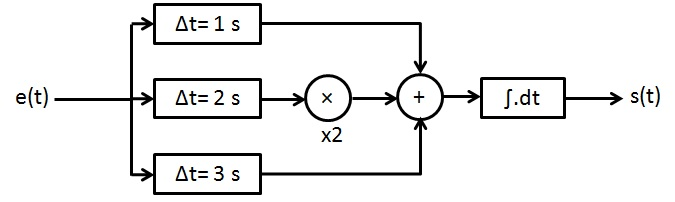
\includegraphics[scale=0.5]{images/Exo_2_6.jpg} 
	\end{figure}
	
	a. Ecrivez la fonction de transfert du système dans le domaine de Laplace.
	
	b. Calculez la réponse indicielle du système. On supposera que les conditions initiales de tous les nœuds internes du système sont nulles. 
	
	
	\vspace{1\baselineskip}
	
	\subsubsection{Exercice 6}
	
	On considère un circuit électrique, dont le courant i(t) est donné par l'équation ci-dessous.
	\begin{equation*}
		e(t)=\frac{d^{2}i}{dt^{2}}+7\frac{di}{dt}+10i(t)
	\end{equation*}
	On considère l'excitation suivante $e(t)=6e^{-3t}u(t)$. Les conditions initiales du circuit sont : $i(0) = 3~A$ et $\frac{di}{dt}(0)=3~A/s$.
	
	
	a. Etablir l'expression du courant dans le domaine de Laplace.
	
	b. En déduire l'expression temporelle du courant i(t).
	
	c. Vérifiez, en utilisant les expressions du courant dans le domaine de Laplace, puis dans le domaine temporel, que la condition initiale du courant est respectée. Déterminez ensuite les conditions finales.
	
	\vspace{1\baselineskip}
	
	\textbf{\underline{Correction exercice 6}}\\
	a. A partir de l'équation différentielle et des conditions initiales, la transformée de Laplace est la suivante :
	
	\begin{equation*}
		p^{2}I(p)-pi(0)-i(0)+7pI(p)-7i(0)+10I(p)=\frac{6}{p+3}
	\end{equation*}
	On transforme ensuite cette relation pour exprimer I(p) sous la forme d'une somme d'éléments dont nous disposons l'expression temporelle (par exemple, fonction rationnelle).
	\begin{equation*}
	I(p)\cdot (p^{2}+7p+10)=\frac{6}{p+3}+3(p+8)
	\end{equation*}
	\begin{equation*}
	I(p)\cdot (p+2)(p+5)=\frac{3(p^{2}+11p+26)}{p+3}
	\end{equation*}
	\begin{equation*}
	I(p)=\frac{3(p^{2}+11p+26)}{(p+3)(p+2)(p+5)}
	\end{equation*}
	En utilisant la méthode du cache, on décompose en pôles et résidus l'expression précédente.
	\begin{equation*}
		I(p)=\frac{A}{p+2}+\frac{B}{p+3}+\frac{C}{p+5}
	\end{equation*}
	\begin{equation*}
		(p+2)I(p)=\frac{3(p^{2}+11p+26)}{(p+3)(p+5)}=A+\frac{B(p+2)}{p+3}+\frac{C(p+2)}{p+5}~\rightarrow~p=-2~:~A=\frac{3((-2)^{2}+11\cdot (-2)+26)}{(-2+3)(-2+5)}=8
	\end{equation*}
	\begin{equation*}
	(p+3)I(p)=\frac{3(p^{2}+11p+26)}{(p+2)(p+5)}=\frac{A(p+3)}{p+2}+B+\frac{C(p+3)}{p+5}~\rightarrow~p=-3~:~B=\frac{3((-3)^{2}+11\cdot (-3)+26)}{(-3+2)(-3+5)}=-3
	\end{equation*}
	\begin{equation*}
	(p+5)I(p)=\frac{3(p^{2}+11p+26)}{(p+2)(p+3)}=\frac{A(p+5)}{p+2}+\frac{B(p+5)}{p+3}+C~\rightarrow~p=-5~:~C=\frac{3((-5)^{2}+11\cdot (-5)+26)}{(-5+2)(-5+3)}=-2
	\end{equation*}
	L'expression du courant dans le domaine de Laplace peut s'écrire de la manière suivante :
	\begin{equation*}
		I(p)=\frac{8}{p+2}-\frac{3}{p+3}-\frac{2}{p+5}
	\end{equation*}
	
	\vspace{0.5\baselineskip}
	
	b. A partir de l'expression précédente, on en déduit directement la forme temporelle du courant à l'aide de la table des transformées de Laplace inverse usuelles.
	\begin{equation*}
	i(t)=(8e^{-2t}-3e^{-3t}-2e^{-5t})u(t)
	\end{equation*}
	
	\vspace{0.5\baselineskip}
	
	c. Condition initiale du courant : d'après les propriétés de la transformée de Laplace, on sait que :
	\begin{equation*}
		\lim_{t\rightarrow0^{+}} i(t)=\lim_{p \to +\infty} pI(p)
	\end{equation*}
	On vérifie cette égalité en retrouvant la valeur de la condition initiale du courant.
	\begin{equation*}
		\lim_{t\rightarrow0^{+}} i(t)=\lim_{t\rightarrow0^{+}}(8e^{-2t}-3e^{-3t}-2e^{-5t})u(t)=8-3-2=3~A
	\end{equation*}
	\begin{equation*}
		\lim_{p \to +\infty} pI(p)=	\lim_{p \to +\infty} \frac{8p}{p+2}-\frac{3p}{p+3}-\frac{2p}{p+5}=8-3-2=3~A
	\end{equation*}
	
	Condition finale du courant : d'après les propriétés de la transformée de Laplace, on doit vérifier que :
	\begin{equation*}
	\lim_{t \to +\infty} i(t)=\lim_{p \to 0} pI(p)
	\end{equation*}
	
	On détermine ainsi la valeur finale du courant.
	\begin{equation*}
	\lim_{t \to +\infty} i(t)=\lim_{t \to +\infty}(8e^{-2t}-3e^{-3t}-2e^{-5t})u(t)=0~A
	\end{equation*}
	\begin{equation*}
	\lim_{p \to 0} pI(p)=	\lim_{p \to 0} \frac{8p}{p+2}-\frac{3p}{p+3}-\frac{2p}{p+5}=0~A
	\end{equation*}
	
	
	
	
\end{document}